% !TEX root = owasp-doc.tex

% ================================================
%	OWASP Resources
% ================================================

\headerimage
\chapter{Resources}

\section{OWASP Top 10 for Large Language Model Applications}

\begin{figure}[ht]
  \centering
  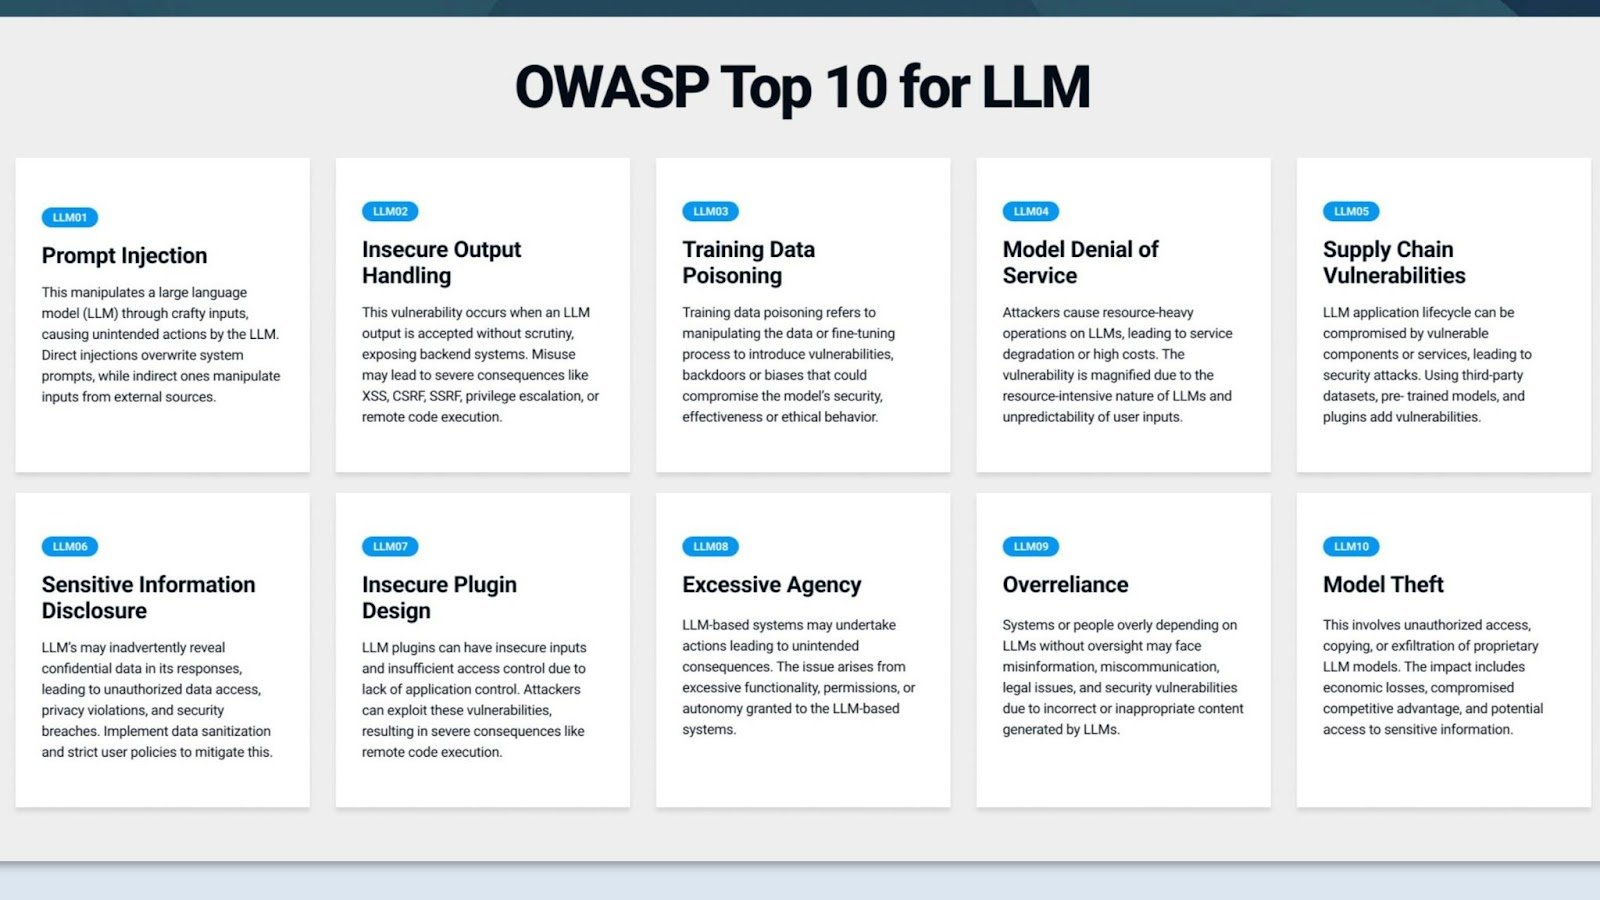
\includegraphics[width=0.8\textwidth]{owasp_top_10_llm_highlevel}
  \caption{Image of OWASP Top 10 for Large Language Model Applications}
  \label{fig:owasp-top-10-llm-highlevel}
\end{figure}

\clearpage
\section{OWASP Top 10 for Large Language Model Applications Visualized}

\begin{figure}[ht]
  \centering
  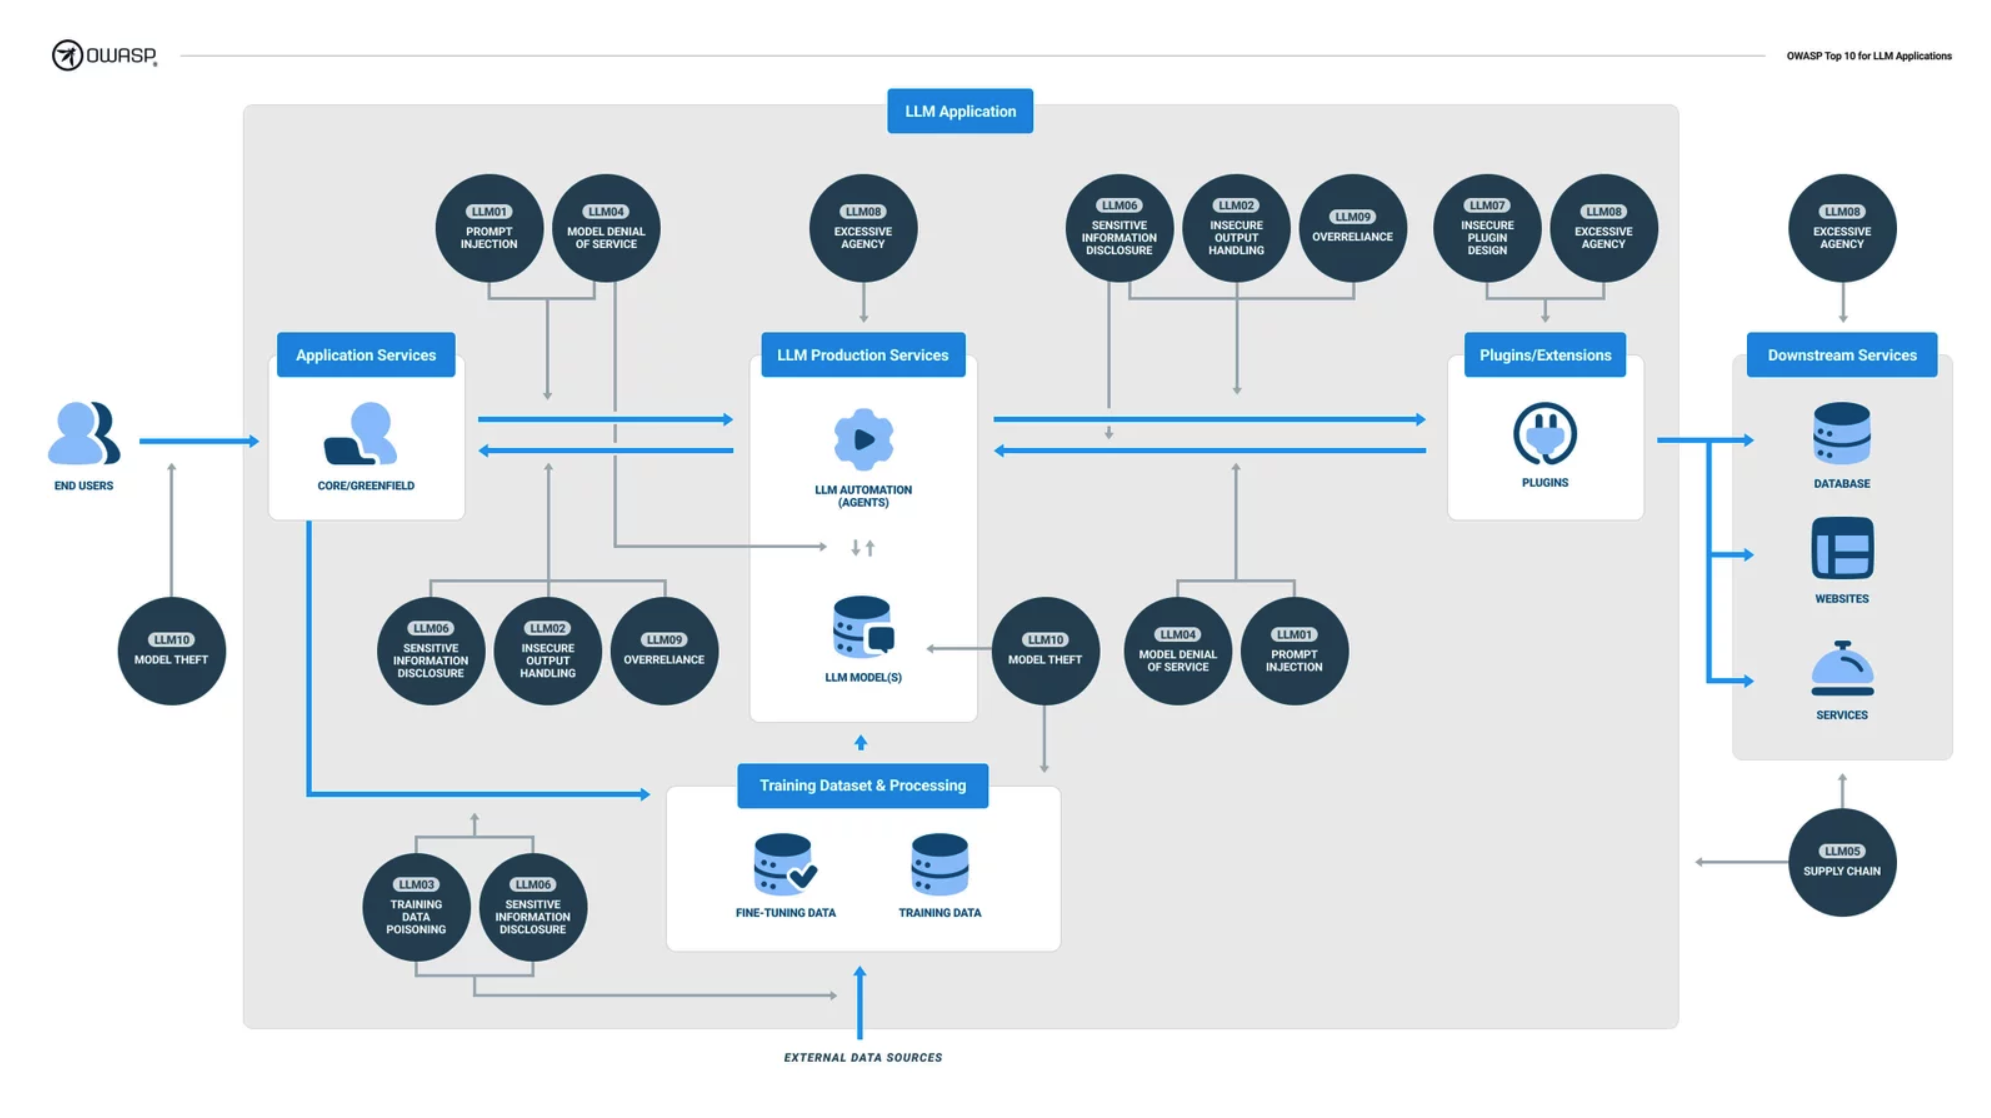
\includegraphics[width=0.8\textwidth]{owasp_top_10_llm_app_arch}
  \caption{Image of OWASP Top 10 for Large Language Model Applications Visualized}
  \label{fig:owasp-top-10-llm-visualized}
\end{figure}

\clearpage
\section{OWASP Resources}

Using LLM solutions expands an organization's attack surface and presents new
challenges, requiring special tactics and defenses. It also poses problems that
are similar to known issues, and there are already established cybersecurity
procedures and mitigations. Integrating LLM cybersecurity with an organization's
established cybersecurity controls, processes, and procedures allows an
organization to reduce its vulnerability to threats. How they integrate with
each other is available at the
\href{https://owasp.org/www-project-integration-standards/}{OWASP Integration Standards}.

%%% TABLE FORMATTING
\setlength\LTleft{0pt}
\setlength\LTright{0pt}
\begin{longtable}[c]{|p{0.25\textwidth}|p{0.25\textwidth}|p{0.35\textwidth}|}
  %%% Header and footer information
  \hline
  \rowcolor{owasplightpurple}
  \textbf{OWASP Resource} &
  \textbf{Description} &
  \textbf{Why It Is Recommended \& Where To Use It} \\
  \hline
  \endfirsthead
  \hline
  \rowcolor{owasplightpurple}
  \textbf{OWASP Resource} &
  \textbf{Description} &
  \textbf{Why It Is Recommended \& Where To Use It} \\
  \hline
  \endhead
  \endfoot
  %%% TABLE DATA GOES HERE
  \href{https://owasp.org/www-project-samm/}{OWASP SAMM} & Software Assurance Maturity Model & Provides an effective and measurable way to analyze and improve an organization's secure development lifecycle. SAMM supports the complete software lifecycle. It is interative and risk-driven, enabling organizations to identify and prioritize gaps in secure software development so resources for improving the process can be dedicated where efforts have the greatest improvement impact. \\
  \hline
  \href{https://owasp.org/www-project-ai-security-and-privacy-guide/}{OWASP AI Security and Privacy Guide} & Software Assurance Maturity Model & Provides an effective and measurable way to analyze and improve an organization's secure development lifecycle. SAMM supports the complete software lifecycle. It is interative and risk-driven, enabling organizations to identify and prioritize gaps in secure software development so resources for improving the process can be dedicated where efforts have the greatest improvement impact. \\
  \hline
  \href{https://owasp.org/www-project-samm/}{OWASP SAMM} & Software Assurance Maturity Model & Provides an effective and measurable way to analyze and improve an organization's secure development lifecycle. SAMM supports the complete software lifecycle. It is interative and risk-driven, enabling organizations to identify and prioritize gaps in secure software development so resources for improving the process can be dedicated where efforts have the greatest improvement impact. \\
  \hline
  \href{https://owasp.org/www-project-samm/}{OWASP SAMM} & Software Assurance Maturity Model & Provides an effective and measurable way to analyze and improve an organization's secure development lifecycle. SAMM supports the complete software lifecycle. It is interative and risk-driven, enabling organizations to identify and prioritize gaps in secure software development so resources for improving the process can be dedicated where efforts have the greatest improvement impact. \\
  \hline
  \href{https://owasp.org/www-project-samm/}{OWASP SAMM} & Software Assurance Maturity Model & Provides an effective and measurable way to analyze and improve an organization's secure development lifecycle. SAMM supports the complete software lifecycle. It is interative and risk-driven, enabling organizations to identify and prioritize gaps in secure software development so resources for improving the process can be dedicated where efforts have the greatest improvement impact. \\
  \hline
  \href{https://owasp.org/www-project-samm/}{OWASP SAMM} & Software Assurance Maturity Model & Provides an effective and measurable way to analyze and improve an organization's secure development lifecycle. SAMM supports the complete software lifecycle. It is interative and risk-driven, enabling organizations to identify and prioritize gaps in secure software development so resources for improving the process can be dedicated where efforts have the greatest improvement impact. \\
  \hline
  \href{https://owasp.org/www-project-samm/}{OWASP SAMM} & Software Assurance Maturity Model & Provides an effective and measurable way to analyze and improve an organization's secure development lifecycle. SAMM supports the complete software lifecycle. It is interative and risk-driven, enabling organizations to identify and prioritize gaps in secure software development so resources for improving the process can be dedicated where efforts have the greatest improvement impact. \\
  \hline
  \href{https://owasp.org/www-project-samm/}{OWASP SAMM} & Software Assurance Maturity Model & Provides an effective and measurable way to analyze and improve an organization's secure development lifecycle. SAMM supports the complete software lifecycle. It is interative and risk-driven, enabling organizations to identify and prioritize gaps in secure software development so resources for improving the process can be dedicated where efforts have the greatest improvement impact. \\
  \hline
  \href{https://owasp.org/www-project-samm/}{OWASP SAMM} & Software Assurance Maturity Model & Provides an effective and measurable way to analyze and improve an organization's secure development lifecycle. SAMM supports the complete software lifecycle. It is interative and risk-driven, enabling organizations to identify and prioritize gaps in secure software development so resources for improving the process can be dedicated where efforts have the greatest improvement impact. \\
  \hline
  \href{https://owasp.org/www-project-samm/}{OWASP SAMM} & Software Assurance Maturity Model & Provides an effective and measurable way to analyze and improve an organization's secure development lifecycle. SAMM supports the complete software lifecycle. It is interative and risk-driven, enabling organizations to identify and prioritize gaps in secure software development so resources for improving the process can be dedicated where efforts have the greatest improvement impact. \\
  \hline
\caption{OWASP Resources}
\label{tab:owasp-resources}
\end{longtable}

\clearpage
\section{MITRE Resources}

The increased frequency of LLM threats emphasizes the value of a
resilience-first approach to defending an organization's attack surface.
Existing TTPS are combined with new attack surfaces and capabilities in LLM
Adversary threats and mitigations. MITRE maintains a well-established and
widely accepted mechanism for coordinating opponent tactics and procedures
based on real-world observations.

Coordination and mapping of an organization's LLM Security Strategy to MITRE
ATT\&CK and MITRE ATLAS allows an organization to determine where LLM Security
is covered by current processes such as API Security Standards or where
security holes exists.

MITRE ATT\&CK (Adversarial Tactics, Techniques, and Common Knowledge) is a
framework, collection of data matrices, and assessment tool that was made by
the MITRE Corporation to help organizations figure out how well their
cybersecurity works across their entire digital attack surface and find holes
that had not been found before. It is a knowledge repository that is used all
over the world. The MITRE ATT\&CK matrix contains a collection of strategies
used by adversaries to achieve a certain goal. In the ATT\&CK Matrix, these
objectives are classified as tactics. The objectives are outlined in attack
order, beginning with reconnaissance and progressing to the eventual goal of
exfiltration or impact.

MITRE ATLAS, which stands for "Adversarial Threat Landscape for Artificial
Intelligence Systems," is a knowledge base that is based on real-life examples
of attacks on machine learning (ML) systems by bad actors. ATLAS is based on the
MITRE ATT\&CK architecture, and its tactics and procedures complement those
found in ATT\&CK.

\begin{table}[h]
\begin{tabularx}{\textwidth} {
  | >{\raggedright\arraybackslash}X
  | >{\raggedright\arraybackslash}X
  | >{\raggedright\arraybackslash}X | }
 \hline
  \rowcolor{owasplightpurple}
    \textbf{MITRE Resource} & \textbf{Description} & \textbf{Why It Is Recommended \& Where To Use It}   \\
    \hline
    Res1 & Des1  & Why1  \\
    \hline
\end{tabularx}
\caption{OWASP Resources}
\label{tab:mitre-resources}
\end{table}

\clearpage
\section{AI Vulnerability Repositories}

\begin{table}[h]
\begin{tabularx}{\textwidth} {
  | >{\raggedright\arraybackslash}X
  | >{\raggedright\arraybackslash}X | }
 \hline
  \rowcolor{owasplightpurple}
    \textbf{Name} & \textbf{Description}   \\
    \hline
    Res1 & Des1   \\
    \hline
\end{tabularx}
\caption{AI Vulnerability Repositories}
\label{tab:ai-vulnerability-repositories}
\end{table}

\clearpage
\section{AI Procurement Guidance}

\begin{table}[h]
\begin{tabularx}{\textwidth} {
  | >{\raggedright\arraybackslash}X
  | >{\raggedright\arraybackslash}X | }
 \hline
  \rowcolor{owasplightpurple}
    \textbf{Name} & \textbf{Description}   \\
    \hline
    Res1 & Des1   \\
    \hline
\end{tabularx}
\caption{AI Procurement Guidance}
\label{tab:ai-procurement-guidance}
\end{table}
